\documentclass[11pt]{article}

\usepackage[a4paper,margin=0.9in]{geometry}
\usepackage[T1]{fontenc}
\usepackage{lmodern}
\usepackage{graphicx}
\usepackage{float}
\usepackage{needspace}
\usepackage{booktabs}
\usepackage{tabularx}
\usepackage{xcolor}
\usepackage{enumitem}
\usepackage{tikz}
\usetikzlibrary{arrows.meta,positioning,fit,backgrounds}
\usepackage[colorlinks=true,linkcolor=blue!60!black,urlcolor=blue!60!black]{hyperref}

\setlength{\parskip}{0.45em}
\setlength{\parindent}{0pt}
\setlength{\emergencystretch}{2em}
\setlist{nosep,leftmargin=1.3em}

\definecolor{cApp}{HTML}{1F5C99}
\definecolor{cOO}{HTML}{0E7C66}
\definecolor{cExt}{HTML}{9E3B2E}
\definecolor{cUser}{HTML}{4B5563}

% A screenshot slot: shows the image once it exists in figures/, otherwise a
% framed note saying which screenshot belongs there.
\newcommand{\shot}[3]{%
  \begin{figure}[H]
    \centering
    \IfFileExists{figures/#1}%
      {\includegraphics[width=\linewidth]{figures/#1}}%
      {\fbox{\parbox[c][4.5cm][c]{0.92\linewidth}{\centering\small\textit{Screenshot pending:} \texttt{\detokenize{figures/#1}}}}}
    \caption{#2}
    \label{#3}
  \end{figure}}

\title{\vspace{-1.2em}\textbf{Lab 8: OpenTelemetry}\\[0.2em]
\large Observability for the AI-based Village Pond Planning System}
\author{Rishi Kharya}
\date{\today}

\begin{document}
\maketitle
\vspace{-1em}

\begin{center}
\fbox{\parbox{0.92\linewidth}{\small
\textbf{Application (sys4):}~\url{http://10.1.75.79:5228/}\\[1pt]
\textbf{Observability backend -- OpenObserve (sys2):}~\url{http://10.1.75.79:5226/}\\[1pt]
\textbf{Source code:}~\url{https://github.com/krish1809/village-pond} \quad(\texttt{backend/telemetry.py})
}}
\end{center}

\section{What I set out to do}

For this lab I added OpenTelemetry to my Assignment~1 project, the Village Pond
Planning System. It is a FastAPI service that takes an area selected on a map,
downloads an elevation model for it from OpenTopography, routes water across the
terrain, ranks candidate pond sites, looks up rainfall from Open-Meteo and works out
how much water each pond could collect. That is a good fit for observability: a
single request crosses two external services and around ten processing stages,
and when it is slow or fails, the plain request log does not say why.

The goal was to capture all three kinds of telemetry --- \textbf{traces},
\textbf{metrics} and \textbf{logs} --- from the real running application on the lab
server, send them to a proper backend, and then actually use what was collected to
explain how the system behaves.

\section{How the implementation is organised}

\begin{figure}[htbp]
\centering
\resizebox{\linewidth}{!}{%
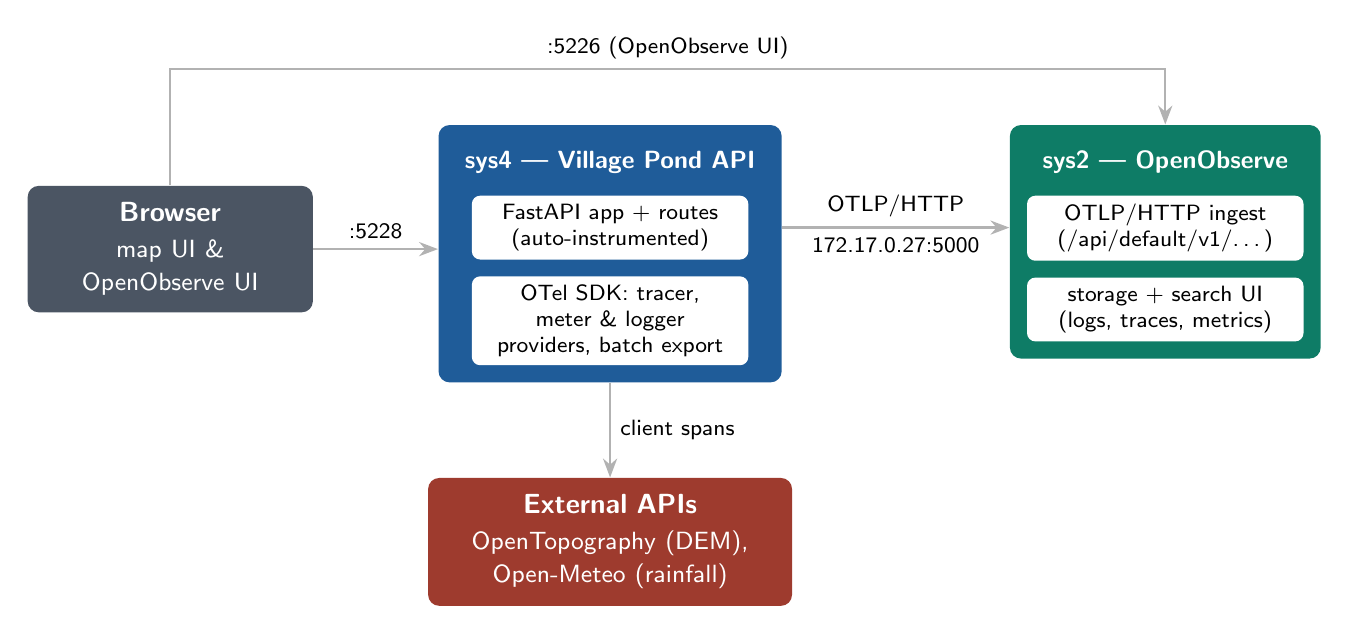
\begin{tikzpicture}[
  font=\sffamily,
  box/.style={rounded corners=4pt, align=center, inner sep=6pt, text=white, minimum height=12mm},
  sub/.style={rounded corners=3pt, align=center, inner sep=3pt, fill=white, text=black, font=\footnotesize\sffamily, text width=3.3cm},
  arr/.style={-{Stealth[length=2.4mm]}, thick, gray!60},
  lab/.style={font=\footnotesize\sffamily, text=black, align=center},
]
\node[box, fill=cUser, text width=3.2cm] (user) {\textbf{Browser}\\[1pt]\small map UI \& OpenObserve UI};

\node[text=white, font=\bfseries\sffamily\small, right=18mm of user, yshift=11mm] (t4) {sys4 --- Village Pond API};
\node[sub, below=1.5mm of t4] (fast) {FastAPI app + routes\\(auto-instrumented)};
\node[sub, below=2mm of fast] (sdk) {OTel SDK: tracer, meter \& logger providers, batch export};
\begin{scope}[on background layer]
\node[fit=(t4)(fast)(sdk), box, fill=cApp, inner sep=6pt] (sys4) {};
\end{scope}

\node[text=white, font=\bfseries\sffamily\small, right=34mm of t4] (t2) {sys2 --- OpenObserve};
\node[sub, below=1.5mm of t2] (ingest) {OTLP/HTTP ingest\\(/api/default/v1/\ldots)};
\node[sub, below=2mm of ingest] (store) {storage + search UI\\(logs, traces, metrics)};
\begin{scope}[on background layer]
\node[fit=(t2)(ingest)(store), box, fill=cOO, inner sep=6pt] (sys2) {};
\end{scope}

\node[box, fill=cExt, text width=4.2cm, below=12mm of sys4] (ext) {\textbf{External APIs}\\[1pt]\small OpenTopography (DEM), Open-Meteo (rainfall)};

\draw[arr] (user.east) -- node[lab, above]{:5228} (user.east -| sys4.west);
\draw[arr] (sys4.east |- fast) -- node[lab, above]{OTLP/HTTP}node[lab, below]{172.17.0.27:5000} (sys2.west |- fast);
\draw[arr] (sys4.south) -- node[lab, right]{client spans} (ext.north);
\draw[arr] (user.north) |- node[lab, pos=0.75, above]{:5226 (OpenObserve UI)} ([yshift=7mm]sys2.north) -- (sys2.north);
\end{tikzpicture}}
\caption{Where the telemetry comes from and where it goes. The app on sys4 exports
over the internal lab network to OpenObserve on sys2; I view the data in the browser
through sys2's forwarded port.}
\label{fig:arch}
\end{figure}

I kept the observability code separate from the analysis code. A single new module,
\texttt{backend/\allowbreak telemetry.py}, installs the OpenTelemetry SDK once when the app
starts. The rest of the code only talks to the OpenTelemetry \emph{API}
(\texttt{opentelemetry.trace} and \texttt{opentelemetry.metrics}), which does
nothing until the SDK is installed. This is the pattern OpenTelemetry recommends for
instrumenting existing code, and it had a practical benefit: my 71 existing tests
never install the SDK, so they ran unchanged.

Everything is exported as \textbf{OTLP over HTTP} and configured only through the
standard environment variables (\texttt{OTEL\_EXPORTER\_OTLP\_ENDPOINT},
\texttt{OTEL\_EXPORTER\_OTLP\_HEADERS}, \texttt{OTEL\_SERVICE\_NAME}). The code has
no idea which backend is on the other end, so OpenObserve could be swapped for
Jaeger, Grafana Tempo or an OpenTelemetry Collector without touching the
application. If no endpoint is set, telemetry simply stays off.

\subsection*{Deployment on the lab systems}
The lab gave us four small containers, each capped at 512\,MB of RAM, with one port
per container forwarded to the outside. The app already ran on sys4. I put the
observability backend on \textbf{sys2}, the container with the most free memory and
an unused forwarded port, so the two would not compete for sys4's 512\,MB. The
containers share an internal Docker network, so sys4 exports straight to
\texttt{172.17.0.27:5000}, while I open the OpenObserve UI from my laptop through
\url{http://10.1.75.79:5226/}. OpenObserve is a single binary that ingests and
displays all three signals behind one port, which is exactly what a one-port,
low-memory container needs. I started it with small worker and cache limits (the
container reports 120 CPUs, and the defaults size themselves from that). It started at
about 200\,MB and, with the test traffic flowing in, sys2's container stayed at roughly
290\,MB of real (anonymous) memory out of its 512\,MB.

\section{Tools, libraries and backend}

\begin{table}[htbp]
\centering
\small
\begin{tabularx}{\linewidth}{@{}lX@{}}
\toprule
Component & Role \\
\midrule
\texttt{opentelemetry-api} / \texttt{-sdk} 1.45.1 & Tracer, meter and logger providers; batch span and log processors; periodic metric reader \\
\texttt{opentelemetry-exporter-otlp-proto-http} 1.45.1 & Sends spans, metrics and log records as OTLP/protobuf over HTTP \\
\texttt{opentelemetry-instrumentation-fastapi} 0.66b1 & Automatic server span and HTTP metrics for every request \\
OpenObserve v1.1.0 (on sys2) & Backend that stores, searches and visualises logs, traces and metrics; supports SQL and PromQL queries \\
FastAPI + uvicorn on Python 3.14 (sys4) & The instrumented Village Pond API \\
\bottomrule
\end{tabularx}
\caption{Libraries and services used.}
\end{table}

\section{What each signal captures}

\paragraph{Traces.}
The FastAPI instrumentation creates one server span per request (method, route,
status code, duration). Inside it I open a child span for every stage of the
pipeline using a small helper, \texttt{telemetry.stage()}: the elevation download,
contour generation, flow routing, drainage extraction, site ranking, the rainfall
lookup, one span per candidate pond, and the PNG render when an image is requested.
Each span carries attributes that matter for this domain, such as the grid size,
whether the elevation model came from the cache, the rainfall source, and each
candidate's catchment area, pond area and collectable volume. The two calls to
external services get their own \emph{client} spans. I created these by hand instead
of auto-instrumenting \texttt{httpx}, because the OpenTopography URL carries my API
key in its query string; the spans record only the host, path, DEM type and response
status, so the key never reaches the backend. Every response also returns its trace
ID in an \texttt{X-Trace-Id} header, and the web page shows it under the results, so
a slow request seen in the browser can be looked up directly.

\paragraph{Metrics.}
Metrics are pushed every 10 seconds. The FastAPI instrumentation provides HTTP
request duration, request and response size and active requests. I added the
application-specific instruments in Table~\ref{tab:metrics}. The memory gauges were
not an afterthought: with a 512\,MB hard limit, memory is the resource most likely
to take this service down.

\begin{table}[htbp]
\centering
\small
\begin{tabularx}{\linewidth}{@{}llX@{}}
\toprule
Instrument & Type & What it tells me \\
\midrule
\texttt{pond.analyses} & counter & Analyses per endpoint and outcome (ok, invalid\_request, upstream\_error, error) \\
\texttt{pond.pipeline.stage.duration} & histogram & Time spent in each pipeline stage \\
\texttt{pond.dem.requests} & counter & Elevation requests served from the cache vs.\ fetched \\
\texttt{pond.upstream.errors} & counter & Failures of external services, by service and kind (e.g.\ rate limit) \\
\texttt{pond.rainfall.lookups} & counter & Rainfall from the live archive vs.\ the offline fallback \\
\texttt{pond.candidates.found} & histogram & Pond sites returned per analysis \\
\texttt{pond.collectable\_volume} & histogram & Collectable water volume of suggested ponds, by rank \\
\texttt{process.memory.rss} & gauge & Resident memory of the API process \\
\texttt{container.memory} & gauge & Container (cgroup) memory used vs.\ its 512\,MB limit \\
\bottomrule
\end{tabularx}
\caption{Custom metrics added to the application.}
\label{tab:metrics}
\end{table}

\paragraph{Logs.}
The app's Python \texttt{logging} output is bridged to OpenTelemetry with a
\texttt{LoggingHandler}. I log the events that matter --- request received, DEM
ready, analysis complete with the headline result, warnings when a request is
invalid or rainfall falls back to the default, and errors from external services ---
with structured attributes (bounding box, durations, outcome). Because each record
is written inside a span, it carries that span's \texttt{trace\_id} and
\texttt{span\_id} automatically, which is what links a log line to the full trace of
the request that produced it. I deliberately kept the \texttt{httpx} library logger
quiet, since it logs every request URL --- including the one with the API key.

\section{Results from the running system}

All screenshots below are from the deployed application on sys4, exporting to
OpenObserve on sys2. The traffic was a mix of real analyses: contour-file uploads,
map-area analyses (one fresh download and several cached repeats), PNG renders and
deliberately invalid requests, plus one analysis run from the browser at the end.

\needspace{12\baselineskip}
\subsection*{Traces}

\shot{traces_list.png}{Traces view in OpenObserve, filtered with
\texttt{service\_name='village-pond-api'} and sorted by duration. The panels at the
top show request rate, errors and a duration heat map over the last hour; below,
each row is one request with its span count. 47 traces were recorded. The
durations separate the request types at a glance: the one area analysis that had to
download a fresh elevation model (14.59\,s, 12 spans), area analyses that also
rendered a PNG map (0.73--1.42\,s, 11 spans), contour-file uploads (0.77--0.97\,s,
8 spans) and cached repeats of the same area (0.17--0.25\,s, 10 spans). The five
``error traces'' are the deliberately invalid requests, whose
\texttt{pond.dem\_fetch} span recorded the bounding-box exception.}{fig:traces}

\shot{trace_waterfall.png}{Waterfall of the slowest trace, the uncached
\texttt{POST /analyzeArea} (trace \texttt{133e6f54\ldots}). The tree shows the
server span, the nine pipeline-stage spans as its children, and the two
\emph{client} spans for the external services, labelled with their peer service
(\texttt{opentopography}, \texttt{open-meteo}). \texttt{pond.dem\_fetch} and its
child \texttt{GET opentopography globaldem} fill almost the whole bar (13.38\,s of
14.59\,s); the rainfall lookup takes 1.02\,s, and contours, flow routing, drainage,
ranking and the three candidate spans are thin slivers totalling about
0.16\,s.}{fig:waterfall}

\shot{span_attributes.png}{Attributes of the \texttt{GET opentopography globaldem}
client span from the same trace. It records the HTTP method, the server
(\texttt{portal.opentopography.org}), the DEM type (\texttt{SRTMGL1}), the response
status (200) and body size (26\,464 bytes) and the duration (13.37\,s). Resource
attributes added by the SDK identify where the span came from:
\texttt{service\_name=village-pond-api}, version 0.3.0,
\texttt{deployment\_environment\_name=lab-sys4} and host \texttt{stu37\_sys4}.
There is no URL query string in the span, so the API key never leaves the
server.}{fig:attrs}

\needspace{12\baselineskip}
\subsection*{Logs}

\shot{logs.png}{Logs view, queried with SQL over the \texttt{default} log stream.
The bar chart shows log volume per minute split by severity (INFO in blue, WARN in
orange); 121 records were stored. Every analysis writes the same three lines ---
\emph{request received}, \emph{DEM ready} (grid size and elevation range) and
\emph{analysis complete} (number of sites, time taken and the rank-1 collectable
volume) --- and each carries the \texttt{trace\_id} of its request. The orange row is
a rejected request with an invalid bounding box.}{fig:logs}

\shot{log_details.png}{The WARN record from Figure~\ref{fig:logs} expanded. Besides
the message it holds the structured attributes I attached
(\texttt{outcome=invalid\_request}, \texttt{status\_code=422}), the source location
added by the logging bridge (\texttt{analyze\_area.py}, line 92), the resource
attributes, and the \texttt{trace\_id}/\texttt{span\_id} of the request. The
\emph{View Trace} button uses that ID to open the trace the log line belongs
to.}{fig:logdetail}

\needspace{12\baselineskip}
\subsection*{Metrics}

\shot{metrics_stages.png}{Average duration of each pipeline stage, computed in
PromQL as \texttt{sum by (stage)} of the histogram's \texttt{\_sum} divided by its
\texttt{\_count}. Because the histogram is cumulative, each line is a running average
since the server started. \texttt{dem\_fetch} (red) starts at about 3.3\,s, when the
one 13.4\,s download is averaged with only a few cached requests, and falls to
0.38\,s as cache hits accumulate. \texttt{render\_png} (teal, about 0.83\,s) ends up
as the slowest stage on average, followed by \texttt{parse\_contours} (about 0.4\,s).
All the terrain computation stages stay below 0.08\,s.}{fig:stages}

\shot{metrics_memory.png}{Resident memory of the API process
(\texttt{process\_memory\_rss}, teal) against the container's hard limit
(\texttt{container\_memory\{kind="limit"\}}, red, 512\,MiB), both from the custom
observable gauges. RSS starts at about 150\,MiB after a restart and steps up to
210--250\,MiB as requests arrive, with the largest jumps coming from PNG renders. It
then stays flat, which shows that the in-memory caches are not
leaking.}{fig:memory}

\shot{metrics_outcomes.png}{The \texttt{pond.analyses} counter grouped by endpoint
and outcome (\texttt{sum by (endpoint, outcome)}). Each step is a request. By the end
of the test run there were 30 successful area analyses, 10 successful contour
analyses and 5 area requests rejected as \texttt{invalid\_request}. There were no
\texttt{upstream\_error} outcomes.}{fig:outcomes}

\needspace{12\baselineskip}
\subsection*{From the web page to the trace}

\shot{app_trace_id.png}{The application on sys4 after analysing the sample area
from the browser (84$\times$134 elevation grid, 12.4\,s, three suggested sites). The
results panel shows the request's trace ID,
\texttt{a09f4e7360c43cb47c4918a744a1ad31}, under the DEM and rainfall
summary.}{fig:apptrace}

\shot{app_trace_lookup.png}{The same trace ID opened in OpenObserve. The request took
12.43\,s, and 12.21\,s of that was the OpenTopography download. The rainfall span
took only 122\,$\mu$s this time, because the rainfall for this location was already
in the cache. The trace has 11 spans rather than 12, because a cached rainfall
lookup makes no outgoing call and so has no client span.}{fig:applookup}

\section{What the data told me}

\paragraph{Where the time actually goes.}
Table~\ref{tab:timings} is taken from the trace of the first analysis of the sample
area on sys4. Before instrumenting I would have guessed that flow routing or the
pond search was the expensive part. The trace says otherwise: \textbf{92\% of the
request is waiting for OpenTopography}, the rainfall archive adds another second,
and all of my own computation together takes roughly 0.15\,s. Repeating the same
request returned in about 0.16\,s, because the elevation model was served from the
in-memory cache (the \texttt{dem.cache\_hit} attribute confirms it, and over the
whole test run the \texttt{pond.dem.requests} counter recorded 29 cache hits against
a single miss). Figure~\ref{fig:stages} shows the same thing: the running average of
\texttt{dem\_fetch} falls from 3.3\,s to under 0.4\,s as cached requests arrive.
That figure also taught me something about reading metrics. An average over the
whole run hides the one slow request, so the trace is what shows how slow an uncached
request really is. So the caching I added in the
previous assignment was the right optimisation, and the place to spend any further
effort is the external download, not the algorithms.

\begin{table}[htbp]
\centering
\small
\begin{tabular}{@{}lr@{}}
\toprule
Span & Duration (ms) \\
\midrule
\texttt{POST /analyzeArea} (whole request) & 14\,590 \\
\quad \texttt{pond.dem\_fetch} $\rightarrow$ \texttt{GET opentopography globaldem} & 13\,381 \;(13\,375) \\
\quad \texttt{pond.rainfall} $\rightarrow$ \texttt{GET open-meteo archive} & 1\,017 \;(1\,016) \\
\quad \texttt{pond.contours} & 53 \\
\quad \texttt{pond.flow\_routing} & 46 \\
\quad \texttt{pond.drainage} & 18 \\
\quad \texttt{pond.rank\_candidates} & 3 \\
\quad \texttt{pond.candidate} $\times$3 & 23, 9, 7 \\
\bottomrule
\end{tabular}
\caption{Span durations for one uncached area analysis on sys4.}
\label{tab:timings}
\end{table}

\paragraph{Memory headroom.}
The memory gauges (Figure~\ref{fig:memory}) showed the API starting at about
150\,MiB and rising to about 250\,MiB once a PNG had been rendered, because
matplotlib is only loaded on the first image request. That is a concrete
justification for loading it lazily. It also shows how close an always-loaded
plotting library would bring the service to the 512\,MiB limit, which it shares
with another lab's Node.js server on sys4. The container gauge's \texttt{used}
series read about 440\,MiB at the end of the run. That figure counts the other
process and reclaimable file cache as well, but it still shows that the box has
little room to spare.

\paragraph{Failures are visible instead of silent.}
Some failures in this app are handled gracefully on purpose, which normally makes
them invisible. When the rainfall service fails, the app quietly uses a default
value; I mark that span as an error and log a warning, so a fallback now shows up
in the traces and in \texttt{pond.rainfall.lookups}. When OpenTopography's free
quota (50 requests per day) runs out, the \texttt{pond.upstream.errors} counter
records it with \texttt{kind=rate\_limit}. Invalid requests are counted by outcome
and logged as warnings with the reason, so a burst of bad input is easy to tell apart
from a server fault.

\paragraph{Debugging a single request.}
The most useful workflow turned out to be the simplest: take the trace ID shown on
the web page (or in the \texttt{X-Trace-Id} header), search for it in OpenObserve,
and get both the full span waterfall and every log line from that request
(Figures~\ref{fig:apptrace} and~\ref{fig:applookup}). Going the other way, the
\emph{View Trace} button on a log record (Figure~\ref{fig:logdetail}) jumps from a
warning to the request that caused it. Metrics
answer ``is something wrong and how often?''; the trace for one request answers
``where exactly and why?''; and the logs carry the human-readable detail. Having all
three tied together by the trace ID is what makes OpenTelemetry more than a logging
library.

\section{Problems I ran into}

\begin{itemize}
\item \textbf{Telemetry lost on restart.} My first version flushed the exporters in
an \texttt{atexit} hook, but nothing arrived when the server was stopped. Recent
versions of uvicorn re-raise \texttt{SIGTERM} after shutting down, which kills the
process before \texttt{atexit} runs. Moving the flush into FastAPI's
\texttt{lifespan} shutdown fixed it; I verified that the final batches of traces,
metrics and logs are now sent when the app stops.
\item \textbf{Noisy traces.} A 6\,MB contour upload produced dozens of tiny ASGI
\texttt{http receive} spans that buried the pipeline stages. Excluding the
\texttt{receive}/\texttt{send} sub-spans in the FastAPI instrumentation left a clean
waterfall of seven meaningful spans.
\item \textbf{Secrets in telemetry.} Auto-instrumenting the HTTP client would have
put the OpenTopography API key into span attributes and logs, so I wrote the client
spans by hand and silenced the \texttt{httpx} logger.
\item \textbf{Running a backend in 512\,MB.} OpenObserve sized its worker pools from
the 120 CPUs the container can see, and it refused to start until the admin password
met its complexity rules. Small explicit limits fixed the first, a stronger password
the second.
\end{itemize}

\section{Conclusion}

The Village Pond API now produces traces, metrics and logs through OpenTelemetry,
exported over OTLP from the lab server to an OpenObserve backend on a second lab
server, without slowing requests down (export happens in background batches). The
data was immediately useful: it showed that nearly all of the response time is the
external elevation download rather than my own code, confirmed that caching removes
it, quantified the memory cost of rendering images against the 512\,MB limit, and made
the app's graceful fallbacks visible. Because the instrumentation only depends on the
OpenTelemetry API and standard OTLP, it stays useful whichever backend is used next.

\paragraph{AI tool usage.} I used Claude while working on this lab, mainly to help set
up the OpenTelemetry SDK and the OpenObserve deployment and to track down the
shutdown-flush problem. I reviewed and tested everything and can explain the
implementation and the results myself.

\end{document}
